
\begin{myex}
	
	\textbf{Répartition des voix entre les trois candidats à une élection}
	
	\begin{multicols*}{2}
	
		\begin{center}
			\begin{tabular}{|@{\ }c@{\ }|@{\ }c@{\ }|}
				\hline
				Candidat & Nombre de voix \\ \hline
				Durand & 300  \\ \hline
				Fabre & 150 \\ \hline
				Lebon & 50 \\ \hline
			\end{tabular}
		\end{center}
		
		
		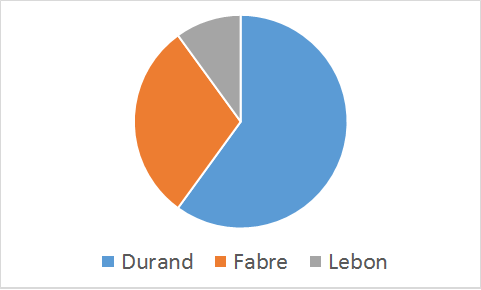
\includegraphics[scale=0.8]{img/sect1}
	\end{multicols*}
	
\end{myex}

